\documentclass[handout,t,compress]{beamer}
\usetheme{Singapore}
\usepackage{etex}
\sloppy
%\usepackage[scaled]{helvet}
%\usepackage{eulervm}

\usepackage{fp-eval}
\usepackage{hyperref}
\usepackage{fancyvrb}
\usepackage{pstricks,pst-node,pst-tree,pst-plot,pst-3dplot,multido}
\usepackage{graphicx}

\usepackage{alltt}


\newcommand{\bframe}[1]{\begin{frame}[fragile]\frametitle{{#1}}}

\newcommand{\bbnf}{\begin{center}\begin{tabular}{rcl}}
\newcommand{\bnf}[2]{#1 & ::= & #2 \\}
\newcommand{\ebnf}{\end{tabular}\end{center}}

\newcommand{\myskip}{\vspace{-1em}\hrulefill}
\newcommand{\myrule}[1]{\vspace{-1ex}\centerline{\rule{#1cm}{1pt}}}
\newcommand{\myline}[1]{\centerline{#1}}
\newcommand{\bkt}[1]{\ensuremath{\langle\mbox{#1}\rangle}}
\newcommand{\br}{\mbox{~}|\mbox{~}}

\definecolor{orange}{rgb}{1,.5,0}
\definecolor{pink}{rgb}{1,.75,.75}
\definecolor{ltblue}{rgb}{.75,.75,1}

\newcommand{\be}{\begin{eqnarray*}}
\newcommand{\ee}{\end{eqnarray*}}

\newcommand{\grph}[2]{
\begin{columns}
\column{0.01\textwidth}
\column{0.6\textwidth}
\begin{pspicture}[showgrid=#1](-2,-2)(5,5)
#2
\end{pspicture}
}

\newcommand{\txt}[1]{
\column{0.4\textwidth}
\rput[bl](0,0){\parbox{\textwidth}{
\footnotesize
\begin{itemize}
#1
\end{itemize}}}
\end{columns}}

\newcommand{\myvec}[1]{
\pstThreeDDot[showpoints=true,drawCoor=true](#1)
\pstThreeDLine[arrows=->,linecolor=blue](0,0,0)(#1)
}

\AtBeginSection[]
{
\bframe{Outline}
\tableofcontents[currentsection]
\end{frame}
}

\title{Notes on Graphs}

\author{CSCI 321}
\institute{WWU}

\begin{document}\small
\psset{arrowscale=2}

\bframe{~}
\titlepage
\end{frame}

\bframe{Navigation Graphs}
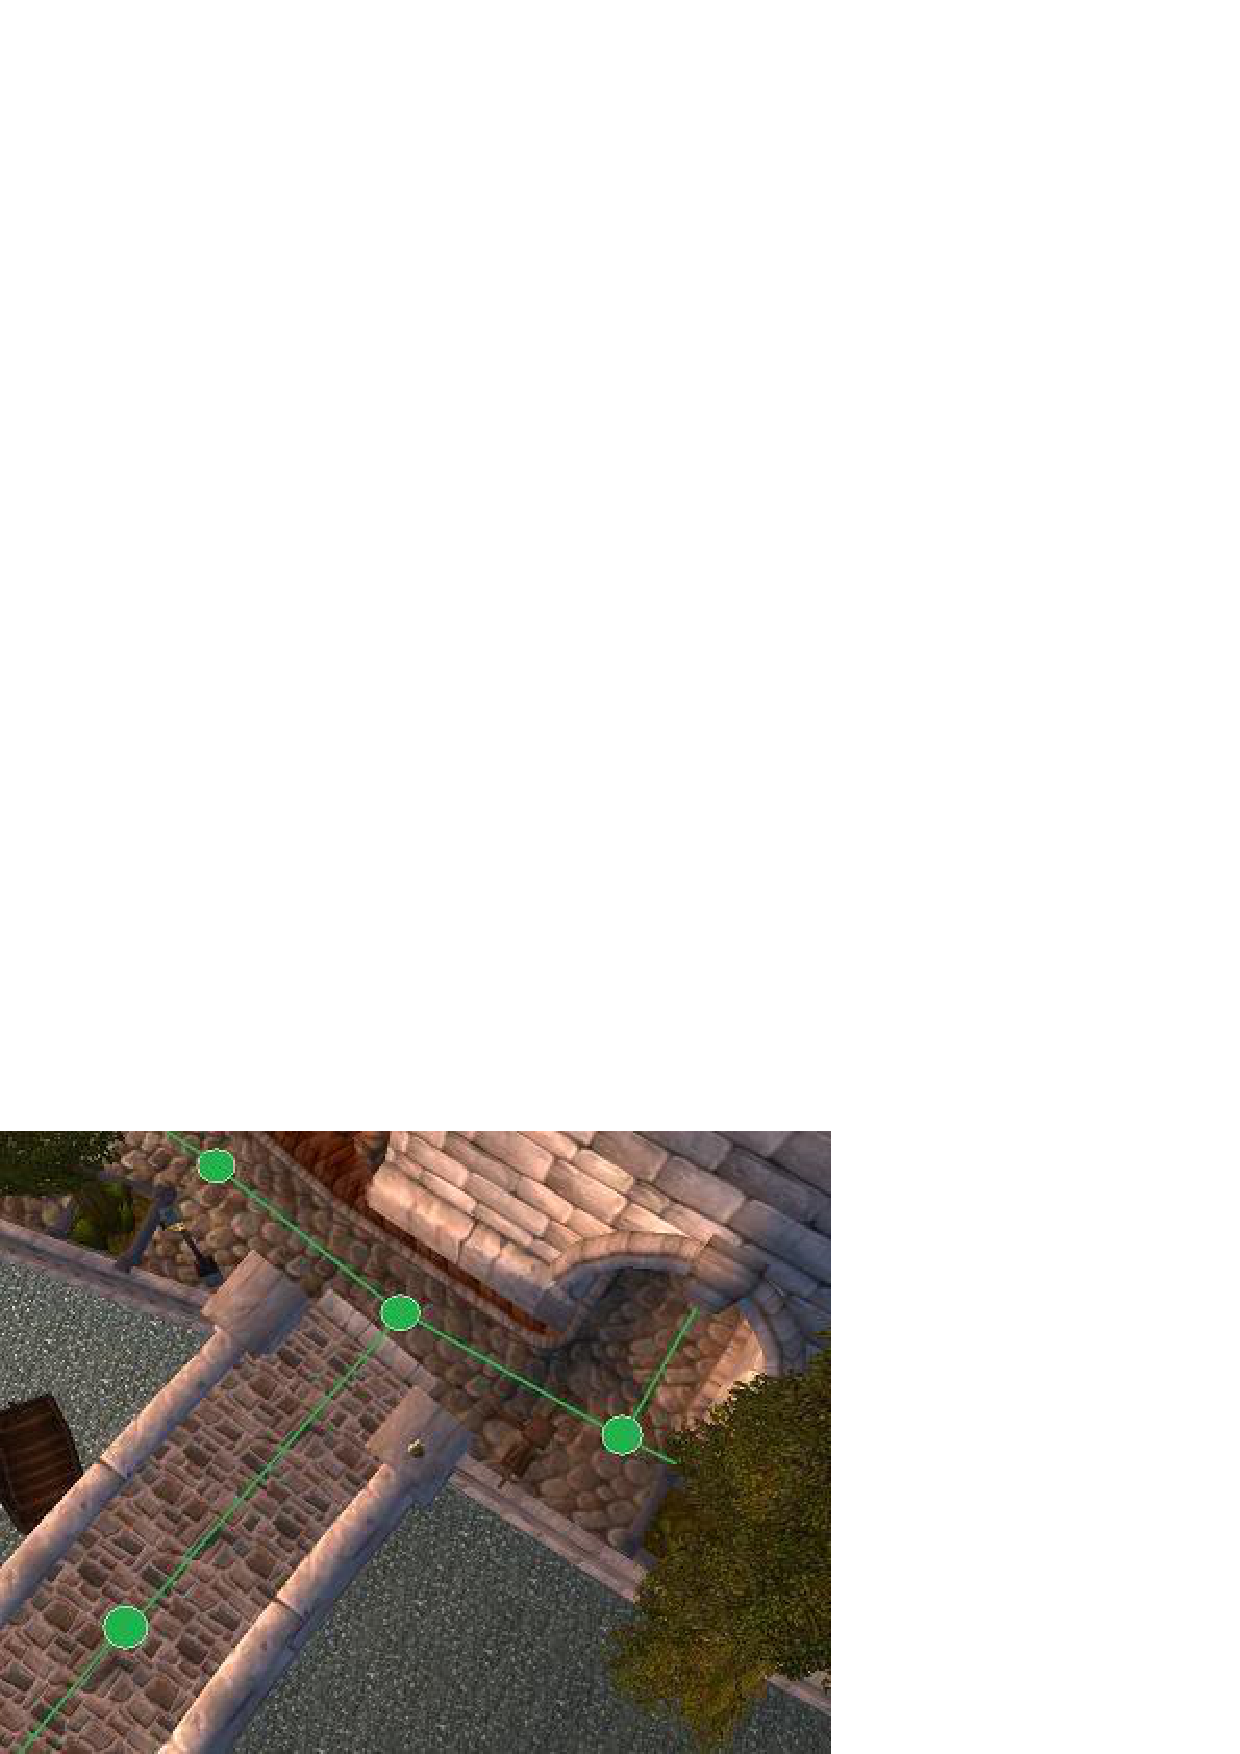
\includegraphics[width=\textwidth]{Stormwind_waypoints.jpg}
\end{frame}

\bframe{Tile Based Games}
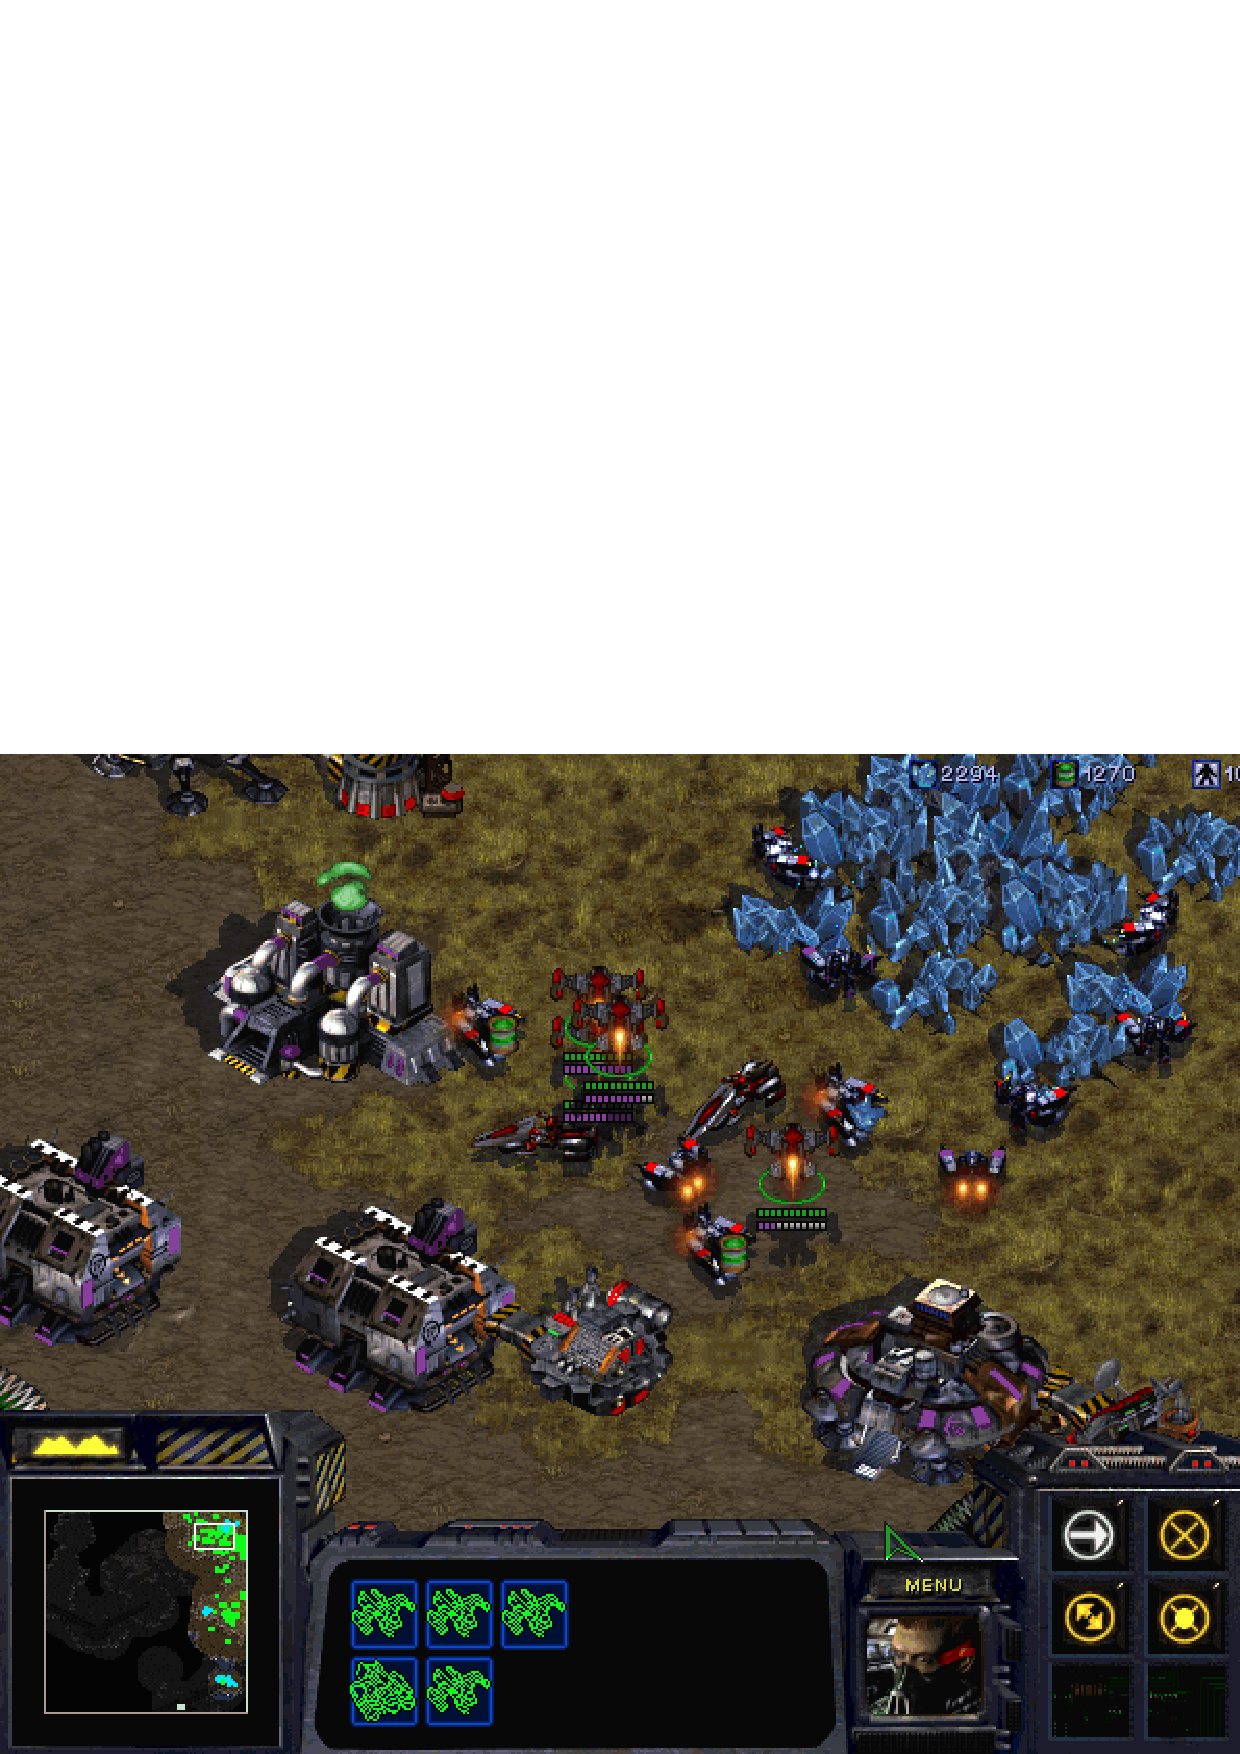
\includegraphics[width=\textwidth]{starcraft.jpg}
\end{frame}


\bframe{Dependency Graphs}
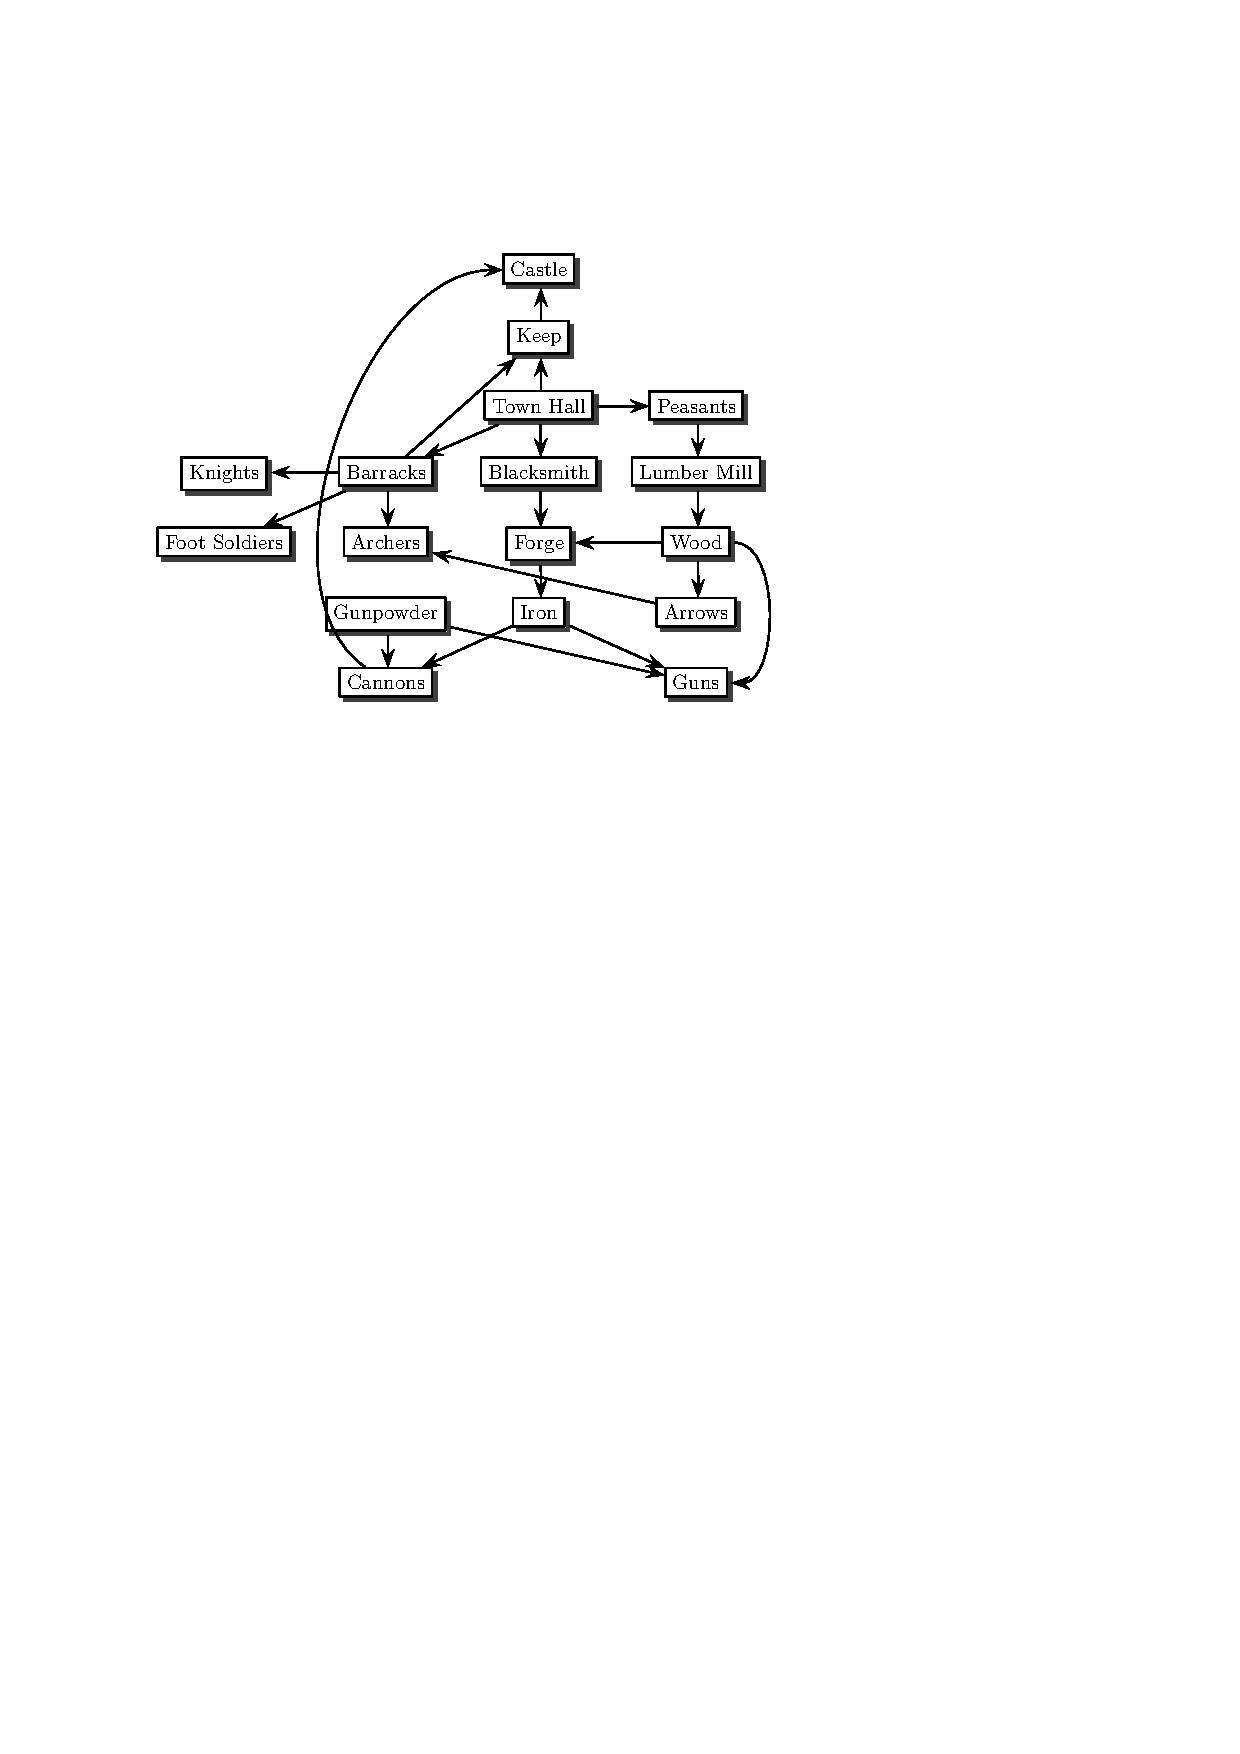
\includegraphics[scale=0.25]{graphsfigure01.png}


\end{frame}


\bframe{Mental Mazes}

\vfill
\begin{center}

\includegraphics[scale=0.25]{graphsfigure02.png}


\end{center}
\vfill

\end{frame}

\bframe{Large Mental Mazes}
\includegraphics{largedialoguemaze.png}
\end{frame}


\bframe{State Graphs}
\includegraphics[scale=0.25]{graphsfigure03.png}


\end{frame}

\bframe{Search}
\begin{itemize}
\item Uninformed search:
\begin{itemize}
\item Depth first search
\item Breadth first search
\item Iterative deepening
\end{itemize}
\item Informed search:
\begin{itemize}
\item Uniform cost (Dijkstra's)
\item Greedy
\item $A^*$ (A-star)
\end{itemize}
\end{itemize}
\end{frame}

\bframe{Resources}
\begin{itemize}
\item \url{http://aima.cs.berkeley.edu/}
\item \url{http://www.barnesandnoble.com/w/introduction-to-game-development-second-edition-steve-rabin/1101415043?ean=9781584506799}
\end{itemize}
\end{frame}

\end{document}


